% vim: set expandtab tabstop=4 shiftwidth=4 textwidth=80:

\documentclass{article}
\usepackage[inner=2.5cm,outer=2.5cm,bottom=1.8cm,top=1.8cm]{geometry}
\usepackage{graphicx}% Include figure files
\graphicspath{ {./graphics/} }
\usepackage{caption}
\usepackage{subcaption}
\usepackage{numprint} % rounds numbers in tables
\npdecimalsign{.}
\nprounddigits{5}
\captionsetup{justification=centering}
\usepackage{wrapfig}
\usepackage{tabu} % for changing individual row fonts
\usepackage{amssymb, amsmath}
\usepackage[mathscr]{euscript}
\usepackage{dsfont}

% for citing things
\usepackage[hyphens]{url}
\usepackage[bookmarks]{hyperref}
%\usepackage{graphicx}
%\usepackage{verbatim}
\hypersetup{
colorlinks,
citecolor=black,
filecolor=black,
linkcolor=black,
urlcolor=black
}
\usepackage{cite}

% nicely written chi
\def\Chi{\raisebox{2pt}{$\chi$}}

%% new column table for tabu to center paragraph cells
% http://tug.org/mail-archives/texhax/2007-March/008042.html
\usepackage{array}
\newcolumntype{C}{>{\centering\arraybackslash}m{2.8cm}} 

% to thicked table lines
\usepackage{booktabs}

% make rows in tables wider
\renewcommand{\arraystretch}{1.4}% Wider

\title{Multi-layer auto-encoders \\
    \large{a CS221 artificial intelligence project}}
    \author{
    Charles Celerier \\
    Computer Science \\
    Stanford \\
    cceleri@cs.stanford.edu
  \and
    Bill Chickering \\
    Computer Science \\
    Stanford \\
    chickering@cs.stanford.edu
}

\begin{document}

\maketitle

This is a short introduction.

\section{Introduction}\label{sec:introduction}

A fundamental challenge to supervised machine learning is that of feature
selection. There exist many strategies for determining a set of variables
derived from an original representation to accurately classify domain data.
Ideally, the selected variables minimize redundant and/or irrelevant information
and thereby reduce the risk of overfitting. Historically, domain experts and
computer scientists have laboriously handcrafted feature sets for a variety of
machine learning problems. These manually engineered features suffer from the
requirements of domain expertise and a great deal of work, and therefore, might
not scale well. Moreover, such feature sets can inadvertently ignore important
structure in the data. These deficiencies can be addressed via unsupervised
feature learning using dimension reduction techniques such as principal
component anaysis (PCA) or factor analysis. Recently it was found that K-means
clustering offers another straightforward method for determining an efficacious
feature space (e.g. the CS221 Visual Cortex programming assigment). In this
report we document a project in which unsupervised feature learning is performed
using autoencoders consisting of multilayer feedforward neural networks.

An autoencoder is a special type of neural network consisting of an input layer,
an output layer, and one or more hidden layers. An autoencoder aims to
approximate the identity function as closely as possible, reproducing the
signals of its input layer at its output layer. By placing constraints on the
network, input signals must be compressed and decompressed using optimized
encodings in order to approximately reproduce the input. Such encodings can then
serve as feature sets in a supervis ed learning problem. The challenge is
training such autoencoders in order to discover the optimal e ncoding for a
particular domain space.

\section{Method}\label{sec:method}

Until recently, the standard approach to training multilayer feedforward neural
networks, such as autoencoders, is to use a variation of the backpropagation
algorithm. We describe this algorithm later in this report. For now, we merely
point out a key feature of the backpropagation algorithm: it attempts to
optimize all weights and biases of a neural network simultaneously. In the case
of large networks containing multiple layers and 1000+ nodes, backpropagation
following random initialization of the parametes can fail due to local minima in
the objective function \ref{art:KL}. A technique pioneered by Hinton et al.
\ref{art:HS} largely overcomes this challenge by "pretraining" individual
restricted Boltzmann machines (RBMs), which can then be "unrolled" to form a
deep, multilayer autoencoder with weights and biases that are close to optimal
prior to running a backpropagation algorithm.

An RBM may be represented as a complete bipartite graph where one set
corresponds to "visible" units $\nu_i$ and the other to "hidden" units $h_j$. We
work with binary RBMs in which each node is either on or off. A weight $w_{ij}$
is associated with each edge that connects a visible unit $\nu_i$ to a hidden
unit $h_j$. Given the state of all visible units, the probability that a hidden
unit is in the "on" state is given by $\sigma\left(b_j +
\sum_i{\nu_iW_{ij}}\right)$, where $\sigma (x)$ is the logistic function $1/(1 +
\mathrm{exp}(-x))$ and $b_j$ is the bias associated with hidden unit $j$.

\section{Results}\label{sec:results}

\begin{figure}[htbp!]
    \centering
    \begin{subfigure}{.45\textwidth}
        \centering
        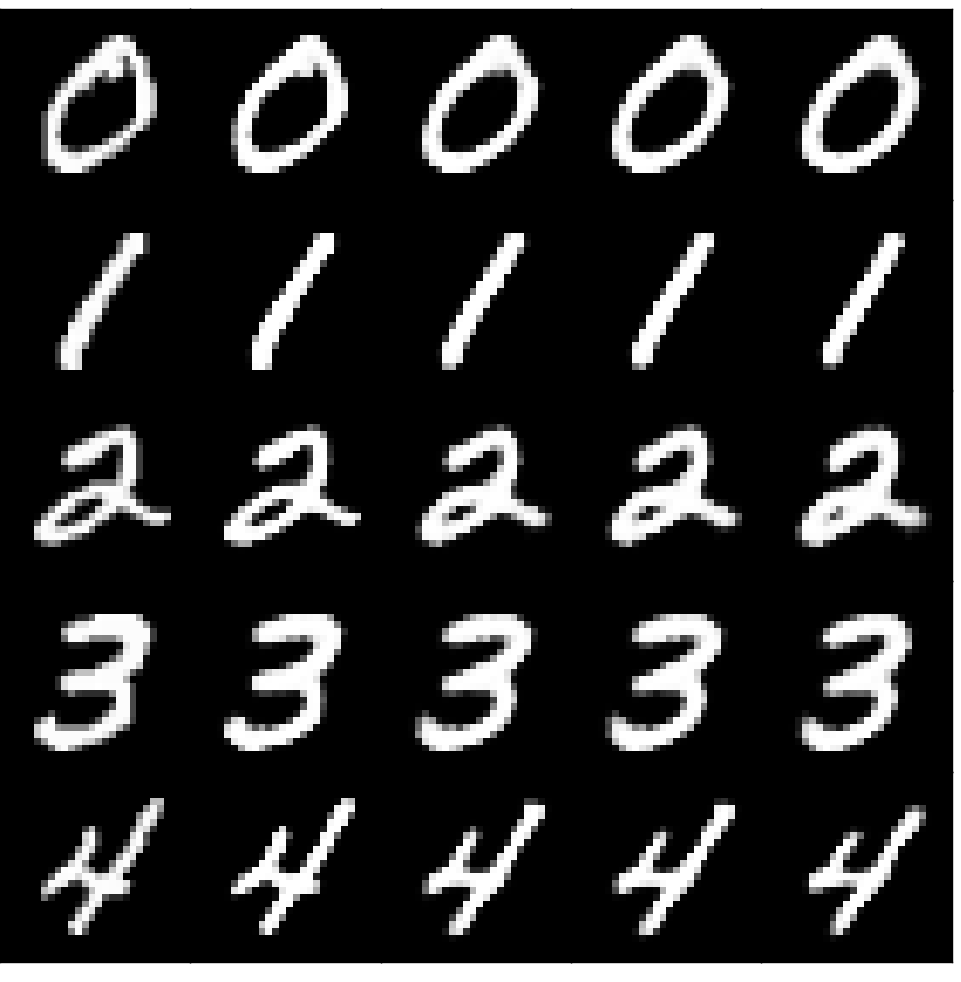
\includegraphics[width=\textwidth]{incremental_0-4.png}
        \caption{Encoding of digits $0-4$ in each layer}
        \label{fig:incremental_0-4}
    \end{subfigure}%
    \quad
    \begin{subfigure}{.45\textwidth}
        \centering
        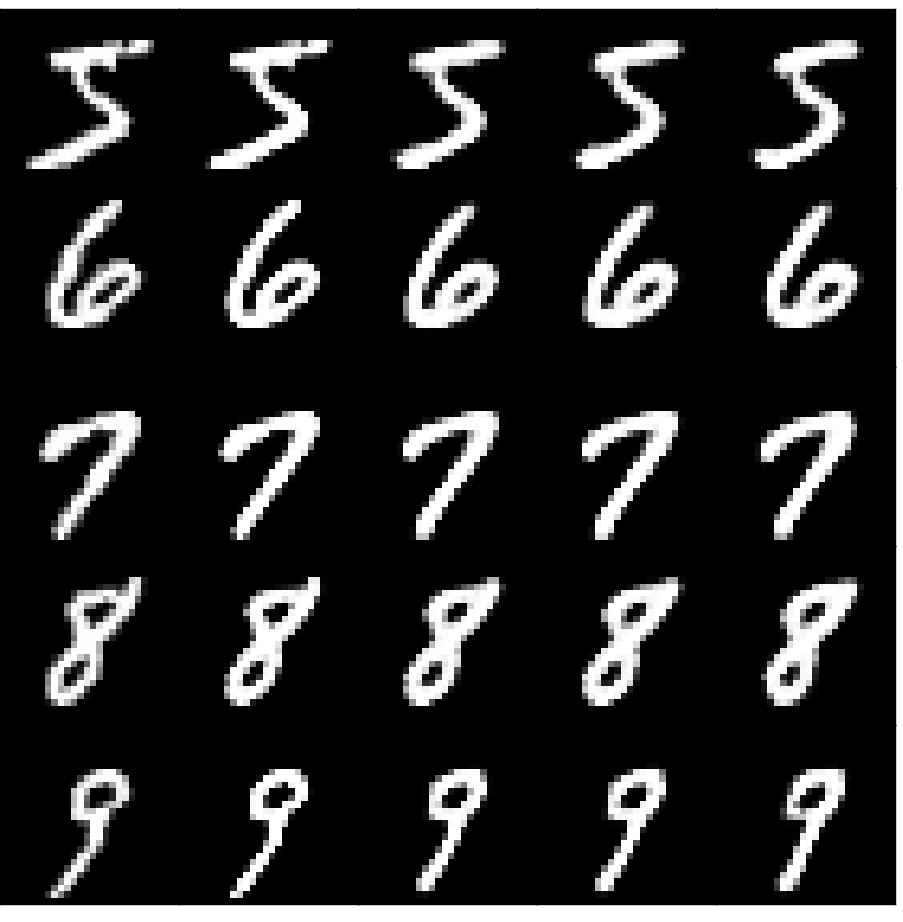
\includegraphics[width=\textwidth]{incremental_5-9.png}
        \caption{Encoding of digits $5-9$ in each layer}
        \label{fig:incremental_5-9}
    \end{subfigure}
\end{figure}

Here's an equation:

\begin{equation}
    \mathscr{C} = \frac{\sum_{q \in Q}\sum_{i=1}^{L_q}\mathds{1}\left\{click\; @\; i \wedge i \leq 16\right\}}{\sum_{q \in Q}\sum_{i=1}^{L_q}\mathds{1}\left\{i \leq 16\right\}},
\end{equation}

\section{Conclusion}\label{sec:conclusion}

\nocite{*}
\bibliography{refs}{}
\bibliographystyle{amsplain}

\end{document}

% vim: set tw=80 ts=4 sw=4 expandtab smarttab:

